\chapter{Survey of morphological metathesis}\label{app:MorMet}

\section{Introduction}
In this appendix I discuss cases of morphological metathesis
not discussed in Chapter \ref{ch:SynchMet}.
That is, all cases of morphological metathesis I know of
outside the Pacific and greater Timor areas.
This appendix is limited to languages where metathesis
has a morphological use in some cases for the simple practical reason that
a list of all metathesis patterns is beyond the scope of this book.

The languages discussed in this appendix are:
Tunisian Arabic (\srf{sec:TunAra}),
Ohlone (\srf{sec:Ohl}), Sierra Miwok (\srf{sec:SieMiw}), Svan (\srf{sec:Sva}),
Alsea (\srf{sec:Als}) and a number of the Salishan languages (\srf{sec:Sal}).
All of these languages, with the exception of Tunisian Arabic
and Svan, are spoken in western America.
A map showing the location of these American languages
is given in \frf{fig:LanWesAmeMorMet}.

\begin{figure}[h]
	\centering
		\setlength\fboxsep{-0.5pt}\setlength\fboxrule{0.75pt}
		\caption{Languages of west America with morphological metathesis}\label{fig:LanWesAmeMorMet}
			\fbox{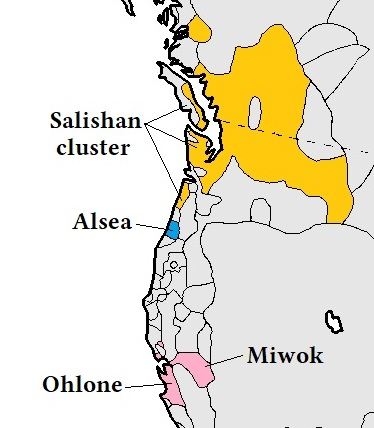
\includegraphics[width=55mm]{WestAmerica-LinLib.jpg}}
\end{figure}


\section{Tunisian Arabic}\label{sec:TunAra}
Metathesis in Tunisian Arabic is described by \cite{kidr86}.
Their discussion begins with the observation that Tunisian Arabic has a process of
phonologically conditioned metathesis (\srf{sec:PhoMet}),
in which the medial CV sequence of a CCVC stem metathesises
before a vowel-initial suffix.
Examples are given in \qf{ex:TunAraMorMet} below.

\begin{exe}
	\ex{CC\sub{2}V\sub{1}C {\ra} CV\sub{1}C\sub{2}C /{\gap}-V \hfill\cite[61]{kidr86}}\label{ex:TunAraMorMet}
	\sn{\gw\begin{tabular}{llcll}
								&Stem							&			&\mc{2}{l}{Suffixed Form}\\
		`palms'			&\it{n\tbr{xa}l}	&{\ra}&\it{n\tbr{ax}l-a}	&`a palm' \\
		`mountain'	&\it{\j\tbr{bə}l}	&{\ra}&\it{\j\tbr{əb}l-i}	&`mountains' \\
		`he wrote'	&\it{k\tbr{tə}b}	&{\ra}&\it{k\tbr{ət}b-u}	&`they wrote' \\
		`month'			&\it{ʃ\tbr{ħa}r}	&{\ra}&\it{ʃ\tbr{aħ}r-iːn}&`two months' \\	
	\end{tabular}}		
\end{exe}

However, there are a number of verbs in which CV {\ra} VC metathesis
alone results in a nominalisation, producing what \citeauthor{kidr86}
call a \it{nomen actionis} (action noun).
Such metathesis only affects words of the shape CCVC.
Examples are given in \qf{ex:TunAraDerMet} below.
%(There is also one example of a metathesis with concurrent apophony of the vowel;
%\it{ħ\tbr{rə}m} `he prohibited' {\ra} \it{ħ\tbr{ar}m} `prohibition'.)

\begin{exe}
	\ex{Nominalising metathesis \hfill\citep[62]{kidr86}}\label{ex:TunAraDerMet}
	\sn{\gw\begin{tabular}{llcll}
										&Verb							&			&Noun&\\
		`he understood'	&\it{f\tbr{hə}m}	&{\ra}&\it{f\tbr{əh}m}		&`understanding'\\
		`he was sick'		&\it{m\tbr{rˁa}ðˁ}	&{\ra}&\it{m\tbr{arˁ}ðˁ}	&`sickness'\\
		`he owned'			&\it{m\tbr{lə}k}		&{\ra}&\it{m\tbr{əl}k}		&`asset'\\
		`he lied'				&\it{k\tbr{ðə}b}		&{\ra}&\it{k\tbr{əð}b}		&`lying'\\
		`he tightened'	&\it{ħ\tbr{sˁa}rˁ}	&{\ra}&\it{ħ\tbr{asˁ}rˁ}	&`act of tightening'\\
		`he blasphemed'	&\it{k\tbr{fɔ}r}		&{\ra}&\it{k\tbr{ɔf}r}		&`blasphemy'\\
		`he prohibited'	&\it{ħ\tbr{rə}m}		&{\ra}&\it{ħ\tbr{ar}m}		&`prohibition'\\
	\end{tabular}}		
\end{exe}

An alternate analysis of the same data would be to identify the nouns as the base
from which verbs are derived by VC {\ra} CV metathesis.
\cite{kidr86} adduce both diachronic evidence
as well as native speaker judgements in favour of their
analysis of metathesis as a nominaliser.

Metathesis is only one of a number of nominalisation strategies in Tunisian Arabic.
Another nominalisation strategy is affixation.
Nominalising affixes include \it{-aːn}, \it{-(j)a},
\it{m(a)-} or a combination of \it{m-{\ldots}-a}.
Examples are given in \qf{ex:TunAraAff} below.
Suffixation with a vowel-initial suffix
also triggers phonologically conditioned metathesis of CCVC roots,
as seen in \qf{ex:TunAraMorMet} above.

\begin{exe}
	\ex{Nominalising affixation \hfill\citep[63f]{kidr86}}\label{ex:TunAraAff}
	\sn{\gw\begin{tabular}{llcll}
										&Verb					&			&Noun										&\\
		`he attached'		&\it{rˁbatˁ}	&{\ra}&\it{rˁabtˁ-\tbr{a}}		&`act of attaching' \\
		`he read'				&\it{qra}			&{\ra}&\it{qraː-\tbr{ja}}			&`reading' \\
		`he blasphemed'	&\it{kfɔr}		&{\ra}&\it{kɔfr-\tbr{aːn}}		&`blasphemy'\footnotemark\\
		`he asked'			&\it{tˁləb}		&{\ra}&\it{\tbr{ma}-tˁləb}		&`request' \\
		`he loved'			&\it{ħabb}		&{\ra}&\it{\tbr{m}-ħabb-\tbr{a}}	&`act of loving' \\
	\end{tabular}}		
\end{exe}
\footnotetext{
Some verbs have multiple nominalising strategies.
The verb \it{kfɔr} `blaspheme' is one such example, either undergoing metathesis,
as shown in \qf{ex:TunAraDerMet}, or suffixation, as shown here in \qf{ex:TunAraAff}.}

Another nominalisation strategy is apophony,
either replacing a short vowel with the equivalent long vowel
or replacing it with a vowel of a different quality.
Examples are given in \qf{ex:TunAraApo} below.

\begin{exe}
	\ex{Nominalising apophony \hfill\citep[64]{kidr86}}\label{ex:TunAraApo}
	\sn{\gw\begin{tabular}{llcll}
									&Verb			&			&Noun				&\\
		`he slept'		&\it{rq\tbr{a}d}&{\ra}&\it{rq\tbr{aː}d}	&`sleep' \\
		`he went mad'	&\it{xb\tbr{ə}l}&{\ra}&\it{xb\tbr{aː}l}	&`going mad' \\
		`he entered'	&\it{dx\tbr{ə}l}&{\ra}&\it{dx\tbr{uː}l}	&`act of entering' \\
		`he swam'			&\it{ʕ\tbr{aː}m}&{\ra}&\it{ʕ\tbr{uː}m}	&`swimming'\\
		`he sold'			&\it{b\tbr{aː}ʕ}&{\ra}&\it{b\tbr{iː}ʕ}	&`(a) sale' \\
	\end{tabular}}		
\end{exe}

The final nominalisation strategy is zero derivation;
that is conversion of a verb into a noun with no phonological change.
Examples are given in \qf{ex:TunAraZerDer} below.

\begin{exe}
	\ex{Zero derivation \hfill\citep[63,65]{kidr86}}\label{ex:TunAraZerDer}
	\sn{\gw\begin{tabular}{lll}
		\it{ʕməl} 	& `he did' {\tl} `deed' \\
		\it{ʕtˁasˁ}	& `sneeze' {\tl} `act of sneezing' \\
		\it{nðˁar} 	& `he saw' {\tl} `seeing' \\
		\it{xbar}		& `he informed' {\tl} `informing' \\
	\end{tabular}}		
\end{exe}

\citet[71]{kidr86} carried out two tests to determine
how productive each of these nominalisation strategies were for CCVC verbs.
In each case metathesis was the most productive nominalisation strategy.

In the first test speakers were presented with ten fictional verbs
and a variety of nominalisations formed according
to each possible process illustrated in \qf{ex:TunAraDerMet}--\qf{ex:TunAraZerDer} above.
Metathesis was the preferred strategy in 8/10 instances
in the first run of this test and was preferred in 9/10 instances in the second run.\footnote{
		The other acceptable nominalisation strategy was suffixation with \it{-aːn}.
		There were also two responses in which either metathesis or suffixation with \it{-aːn}
		were judged acceptable.}

Similar judgements were given for the loan words
\it{nmar} (< French \it{numéroter}) `to number',
\it{mraʃ} (< French \it{marcher}) `to march'
and \it{mrəs} (< French \it{remercier}) `to thank'.
Among loanwords the only exception was \it{bləf} < English \it{bluff},
for which the preferred nominalisation strategy was zero derivation.

The second test \citeauthor{kidr86} carried out
involved choosing either metathesis or zero derivation
as the preferred nominalisation strategy.
In this test 17/18 responses selected metathesis.

In summary, metathesis in Tunisian Arabic is one of several processes
available to nominalise verbs with the structure CCVC.
Metathesis is productive and is the preferred nominalisation strategy.
That metathesis in Tunisian Arabic is associated with other processes
is consistent with the data in Chapter \ref{ch:SynchMet}
in which metathesis is associated with
a large number of additional processes.
%However, in Amarasi most of these processes are consequences of metathesis,
%such as vowel assimilation triggered by metathesis (\srf{sec:VowAss}),
%while in Tunisian Arabic these processes are independent of metathesis,
%with the exception of suffixation triggering metathesis.

\section{Svan}\label{sec:Sva}
Svan is a Kartvelian language of northern Georgia.
Causatives of intransitive verbs are formed in Svan by final VC {\ra} CV metathesis.
Published sources are extremely scarce.
\citet[297]{me97} gives the six examples in \qf{ex:SvaMet} below.
In all six instances metathesis derives a causative from an intransitive verb.\footnote{
		All six examples in \qf{ex:SvaMet} are cited with the prefix \it{li-} of which 
		\citet{me97}, states ``Les exemples ci-dessous sont cités à la forme du nom d’action verbal,
		appelé \emph{masdar}, dont les rôles syntaxiques sont comparables à ceux de l'infinitif du français.'';
		``The examples below are given in the form of a verbal action noun,
		called \emph{masdar}, whose syntactic roles are similar to those of the French infinitive.''}

\begin{exe}
	\ex{Svan causative metathesis \hfill\citep[297]{me97}}\label{ex:SvaMet}
	\sn{\gw\begin{tabular}{llcll}
											&\tsc{intr} 					&			&\tsc{caus}	&\\
		 `go out' 				&\it{li-d\tbr{eg}} 		&{\ra}&\it{li-d\tbr{ge}}		&`extinguish' \\
		 `break (intr.)'	&\it{li-kʷ'\tbr{es'}}	&{\ra}&\it{li-kʷ'\tbr{s'e}}	&`break (tr.)' \\
		 `rot' 						&\it{li-kʷ\tbr{er}} 	&{\ra}&\it{li-kʷ\tbr{re}}		&`make/let rot' \\
		 `come' 					&\it{li-q\tbr{ed}} 		&{\ra}&\it{li-q\tbr{de}}		&`bring, convey' \\
		 `return (intr.)'	&\it{li-t'\tbr{ex}}		&{\ra}&\it{li-t'\tbr{xe}}		&`return (tr.)' \\
		 `get dirty' 			&\it{li-g\tbr{eb}} 		&{\ra}&\it{li-g\tbr{be}}		&`make dirty' \\
	\end{tabular}}		
\end{exe}

\section{Mutsun Ohlone (Costanoan)}\label{sec:Ohl}
Metathesis in the Mutsun variety of Southern Ohlone (a.k.a. Costanoan),
a now extinct language of central California (see \frf{fig:LanWesAmeMorMet}), is described in \cite{ok79}.
The same author also wrote a grammar of the language published as \citet{ok77}.
In both instances data was drawn from material gathered in the
early twentieth century from the last fluent speaker.

Verbs in Mutsun have two stems, called the primary stem and the derived stem.
The main difference between each stem is that the derived stem is consonant final,
while the primary stem can be either vowel final or consonant final.
\cite{ok79} identifies seven types of stems of which stem types II, IV and VII show metathesis.
These three stem types are given in \trf{tab:MutPriDerVerSte}
(the fourth stem type is poorly attested in the data).
In all cases the derived stem is formed from the primary
stem by metathesis of the final VC sequence.

\begin{table}[h]
	\caption[Mutsun primary and derived verb stems]{Mutsun primary and derived verb stems \citep[125]{ok79}}\label{tab:MutPriDerVerSte}
	\centering
		\begin{tabular}{rrllll} \lsptoprule
					&Primary 							&Derived 						& \mc{2}{l}{Examples} 				&Gloss\\ \midrule
			II	&CVCV\sub{2}ːC\sub{3}	&CVCC\sub{3}V\sub{2}& \it{pasiːk-}	& \it{paski-}	&`to greet, visit'\\
			IV	&CVːCV\sub{2}C\sub{3}	&CVCC\sub{3}V\sub{2}& \it{liːwak-}	& 						&`to hide nearby'\\
			VII	&CVCːV\sub{2}C\sub{3}	&CVCC\sub{3}V\sub{2}& \it{liʧːej-}	& \it{liʧje-}	&`to stand'\\
			\lspbottomrule
		\end{tabular}
\end{table}

In most cases the use of each stem is either phonologically or morphemically conditioned.
A phonologically conditioned use is found before suffixes which begin with a consonant cluster
in which case VC {\ra} CV metathesis occurs to prevent a cluster of three consonants surfacing.
Examples include \it{pas\tbr{iːk}} `visit' + \it{-jni} `to come to'
{\ra} \it{pas\tbr{ki}jni} `come to visit'
and \it{liʧː\tbr{ej}} `to stand' + \it{-hte} \tsc{perfective} {\ra}
\it{liʧ\tbr{je}hte} `already assumed a standing position'.

Likewise, word final consonant clusters are disallowed in Mutsun.
As a result derived stems are used before suffixes consisting of a single consonant.
One example is \it{sotː\tbr{er}} `stick out' + \it{-j} \tsc{imperative}
{\ra} \it{sot\tbr{re}j} `stick out [your foot]!' \citep[125]{ok79}.

However, there are also some CV(C) suffixes which only occur with primary stems
and other CV(C) suffixes which only occur with derived stems.
This is a case of morphemically conditioned metathesis (\srf{sec:MorpheConMet}),
in which metathesis is a partial exponent of the morphological
category signalled by the suffix.

Suffixes which take primary stems include the reciprocal suffix \it{-mu}
and the reflexive suffix \it{-pu},
as seen in \it{hiːwo} `scold (s.o.)' + \it{-mu} \tsc{recp} {\ra} \it{hiːwomu} `(they) quarrel' 
and \it{matːal} `face down' + \it{-pu} \tsc{refl} {\ra} \it{matːalpu} `put oneself face down'.
One suffix which takes the derived stem and thus triggers metathesis is \it{-nu} `positional causative',
as seen in \it{matː\tbr{al}} `face down' + \it{-nu} {\ra} \it{mat\tbr{la}nu}
`put (s.o.) face down (into a prone position)' \citep[126]{ok79}.

The morphological function of metathesis comes about because the derived stem
is used in isolation as a non-past tense
and there are a number of cognate nouns
which take the primary stem.
Examples are given in \qf{ex:MutDerMet} below.

\begin{exe}
	\ex{Mutsun derivational metathesis \hfill\citep[127]{ok79}}\label{ex:MutDerMet}
	\sn{\gw\begin{tabular}{llll}
		 					 			&Noun								&Verb							& \\
		 `a cough' 			&\it{toːh\tbr{er}}	&\it{toh\tbr{re}} & `to cough' \\
		 `flute' 				&\it{lulː\tbr{up}}	&\it{lul\tbr{pu}} & `to play the flute' \\
		 `goose' 				&\it{laːl\tbr{ak}}	&\it{lal\tbr{ka}} & `gather geese' \\
		 `nest'					&\it{heːs\tbr{en}}	&\it{hes\tbr{ne}} & `make a nest' \\
		 `pozole (stew)'&\it{pos\tbr{ol}}		&\it{pos\tbr{lo}} & `to make pozole (stew)' \\
	\end{tabular}}		
\end{exe}

Given that Mutsun is now extinct, it is hard to tell exactly how productive metathesis was.
However, the occurrence of the Spanish loanword \it{posol} `pozole (stew)'
with both metathesised  and unmetathesised forms indicates that metathesis was productive.
It is likely that VC {\ra} CV metathesis in Mutsun was used to derive verbs from nouns.\footnote{
		Mutsun \it{posol} is a loan from Spanish \it{pozole}, itself a loan from Nahuatl \it{pozolli}.
		The final final /e/ of the Spanish form has been re-analysed in Mutsun as 
		the object case suffix; \it{posoːl-e} \citep[127, fn.14]{ok77}.}

%The main similarity between the Mutsun Ohlone data and the Amarasi data
%is in the distribution of metathesis.
%In both instances metathesis is phonological
%in some contexts and morphological in others.
\section{Sierra Miwok}\label{sec:SieMiw}
Sierra Miwok is a language of central California
(see \frf{fig:LanWesAmeMorMet}) related to Ohlone (\srf{sec:Ohl}).
My summary of Sierra Miwok metathesis is based on the description in \cite{fr51}.
Like Ohlone, each verb in Sierra Miwok has multiple stems.
There are three derived stems in Sierra Miwok formed from one of
four different shapes of the primary (underlying) stem.
These different shapes are summarised in \trf{tab:SieMiwVerSte}.
on the next page.

\begin{table}[h]
	\caption[Sierra miwok verb stems]{Sierra miwok verb stems\su{†} \citep[94f]{fr51}}\label{tab:SieMiwVerSte}
	\centering
		\begin{threeparttable}[b]
			\begin{tabular}{rccccl}\lsptoprule
					&Primary						&Second				&Third				&Fourth				&\\ \midrule
			I		&CVC\tbr{V}ː\tbr{C}	&CVCVCː				&CVCːVC				&CVC\tbr{CV} 	&\\
					&\it{tujaːŋ-}				&\it{tujaŋː-}	&\it{tujːaŋ-}	&\it{tujŋa-}	& `to jump'\\
			II	&CVC\tbr{CV}				&CVC\tbr{VC}ː	&CVCː\tbr{VC}	&CVCCV 				&\\
					&\it{wɨkt̪ɨ-}				&\it{wɨkɨt̪ː-}	&\it{wɨkːɨt̪-}	&\it{wɨkt̪ɨ-}	&`to burn'\\
			III	&CVCːV							&CVCVʔː				&CVCː\tbr{Vʔ}	&CVC\tbr{ʔV}	&\\
					&\it{hamːe}					&\it{hameʔː-}	&\it{hamːeʔ-}	&\it{hamʔe-}	&`to bury'\\
			IV	&CVːC								&CVCː					&CVCː\tbr{Vʔ}	&CVC\tbr{ʔV}	&\\
					&\it{luːʃ-}					&\it{luʃː-}		&\it{luʃːuʔ-}	&\it{luʃʔu-}	&`to win'\\ \lspbottomrule
			\end{tabular}
			\begin{tablenotes}
				\item [†] Stress in Sierra Miwok falls on the first heavy syllable;
									either VCC, VːC or VCː \citep[7]{fr51}.
									Because it is predictable, I do not indicate its presence in this section.
			\end{tablenotes}
		\end{threeparttable}
\end{table}

The shape of each derived stem is consistent across all four verb classes,
with the exception of the second stem of class IV verbs.
The second derived stem has the shape CVCVCː,
the third stem CVCːVC and the fourth stem CVCCV.

In all cases the final C-slot is filled by a glottal stop
when the root has only two consonants.
Similarly, when the root has only a single vowel the final V-slot is filled
by /u/ after back rounded vowels,
and by /ɨ/ after all other vowels.
Both these facts can be seen with the primary stem \it{luːʃ-} `to win'
with the CVCːVC third stem \it{luʃː\tbr{uʔ}-}
with the final vowel and consonant
occurring to fill the otherwise empty V-slot and C-slot.

Final consonant-vowel metathesis is found in three cases;
between the primary stem of verb class I and the fourth stem,
with VC {\ra} CV metathesis,
and between the primary stem of verb class II
and the second and third derived stems,
with CV {\ra} VC metathesis.
It is also possible to analyse the epenthetic glottal stop as undergoing metathesis
in the third and fourth stems of class III verbs and class IV verbs.

As in Mutsun, some cases of metathesis in Sierra Miwok 
are instances of phonologically conditioned metathesis.
Before a CC initial suffix the fourth stem is used,
thereby avoiding a cluster of three consonants.
One example is the class I stem \it{pol\tbr{a}ː\tbr{ŋ}}
`to stagger' + \it{-jnɨ} \tsc{desiderative}
{\ra} \it{pol\tbr{ŋa}jnɨ} \citep[116]{fr51}.

There are also many instances of morphemically conditioned metathesis
with different suffixes of the same phonological shape occurring with different stems.
Such instances are extremely numerous and I do not provide examples here.

In addition there are also instances
in which metathesis alone serves a a morphological function.
For instance, one nominalisation strategy
for class I verbs is to use the fourth stem.
Examples are given in \qf{ex:SieMiwVerMet} below,
in which nouns are cited with the \tsc{subjective} suffix \it{-ʔ}

\newpage
\begin{exe}
	\ex{Sierra Miwok verbalising metathesis \hfill\citep[149]{fr51}}\label{ex:SieMiwVerMet}
	\sn{\gw\begin{tabular}{lrcll}
								&Verb												&			&Noun									&\\
		`to relate'	&\it{ʔut̪\tbr{e}ː\tbr{n}-}		&{\ra}&\it{ʔut̪\tbr{ne}-ʔ}		&`myth, tale' \\
		`to tell'		&\it{koy\tbr{o}ː\tbr{w}-}		&{\ra}&\it{koy\tbr{wo}-ʔ}		&`words, speech' \\
		`to run'		&\it{hɨw\tbr{a}ː-\tbr{t̪}-}	&{\ra}&\it{hɨw\tbr{t̪a}-ʔ}		&`race' \\
		`to play'		&\it{ʔaw\tbr{i}ː-\tbr{n}-}	&{\ra}&\it{ʔaw\tbr{ni}-ʔ}		&`game' \\
		`to live'		&\it{ʔu{\tS}ːu-}						&{\ra}&\it{ʔu{\tS}ʔu-ʔ}			&`health, well-being: year' \\
		`to come'		&\it{ʔɨnːɨ-}								&{\ra}&\it{ʔɨnʔɨ-ʔ-}				&`way, journey' \\
		`to eat'		&\it{ʔɨwːɨ-}								&{\ra}&\it{ʔɨwʔɨ-ʔ}					&`food' \\
	\end{tabular}}
\end{exe}

The processes in Mutsun Ohlone and Sierra Miwok have much in common,
as might be expected from related languages.
However, in Mutsun Ohlone VC {\ra} CV metathesis is a  verbaliser
while in Sierra Miwok the same process is a nominaliser.

%The Sierra Miwok data has two similarities to Amarasi.
%Firstly, metathesis in Sierra Miwok is phonologically conditioned
%in some contexts and morphological in others.
%Secondly, metathesis in Sierra Miwok interacts with empty C-slots and empty V-slots.
%In Sierra Miwok empty C-slots and V-slots are filled by default segments
%which then metathesise with each other or with specified segments.
%
%In Amarasi, empty C-slots also occur and metathesise with filled V-slots
%triggering processes such as consonant insertion and vowel assimilation.
%The way empty C-slots interact with Amarasi metathesis is discussed in \srf{sec:ThePhoRul}
%and evidence for positing empty C-slots is presented in \srf{sec:EmpCSlo}.

\section{Alsea}\label{sec:Als}
Alsea is a now extinct language of the Oregon coast (see \frf{fig:LanWesAmeMorMet}).
The only consonants which participate in metathesis in Alsea are sonorants.
Metathesis in Alsea is mostly morphemically conditioned (\srf{sec:MorpheConMet}).
One suffix which triggers metathesis is the third person object imperative suffix \it{-t}.
Examples are given in \qf{ex:AlsMorphemicMet} below
in which the metathesised stems on the right
can be compared with unmetathesised counterparts on the left.

\begin{exe}
	\ex{Alsea morphemically conditioned metathesis \hfill\citep[8f]{bu07}}\label{ex:AlsMorphemicMet}
		\sn{\stl{0.3em}\gw\begin{tabular}{lrll}
		`had closed it'				&\it{t\tbr{mú}s-sa-nχ}		&\it{t\tbr{úm}s-t}		&`close it!'\\
		`agreed to it'				&\it{t'\tbr{má}s-sal-tχ}	&\it{t'\tbr{ám}s-t}		&`finish it!'\\
		`had been sliding'		&\it{st\tbr{lá}k-sal-tχ}	&\it{st\tbr{ál}k-t}		&`slide it!'\\
		`is packing'					&\it{ʦu\tbr{lá}q'n-tχ}		&\it{ʦu\tbr{ál}q'n-t}	&`pack it!'\\
		`is close to shore'		&\it{t\tbr{lú}qʷ'-χ}			&\it{t\tbr{úl}qʷ'-t}	&`bring it close to shore!'\\
		`is in act of hiding'	&\it{p\tbr{yá}χ-aw-tχ}		&\it{p\tbr{áy}X-t}		&`hide it!'\\
		`had pierced'					&\it{qɬ\tbr{jú}t-sal}			&\it{qɬ\tbr{új}-t}		&`prick him!'\\
	\end{tabular}}		
\end{exe}

That this metathesis is not conditioned by the phonological shape of the suffix
is shown by the contrast between suffixes with an identical form,
one of which triggers metathesis while the other does not.
The intransitive imperative suffix \it{-χ} triggers metathesis
while the completive realis \it{-χ} suffix does not trigger metathesis.
Examples are given in \qf{ex:AlsMorphemicMet2} below.

\begin{exe}
	\ex{Alsea morphemically conditioned metathesis \hfill\citep[8f]{bu07}}\label{ex:AlsMorphemicMet2}
	\sn{\gw\begin{tabular}{lrll}
											&\tsc{cmpl.rl}			&\tsc{intr.imp}		& \\
		`dances with them'&\it{k\tbr{ná}χ-χ}	&\it{k\tbr{án}χ-χ}&`dance with them!' \\
		`are lying in bed'&\it{ʦ\tbr{nú}s-χ}	&\it{ʦ\tbr{ún}s-χ}&`lie down!' \\
		`is hiding'				&\it{p\tbr{já}χ-χ}	&\it{p\tbr{áj}χ-χ}&`hide!' \\
		`is floating'			&\it{ʦp\tbr{jú}t-χ}	&\it{ʦp\tbr{új}t-χ}&`float!' \\
	\end{tabular}}		
\end{exe}

In addition to such morphemically conditioned metathesis there are also hints that
Alsea had a process of morphological metathesis which signalled aspect.
\cite{bu07} gives three potential examples, given in \qf{ex:AlsMorMet} below.

\begin{exe}
	\ex{Alsea morphological metathesis \hfill\citep[10]{bu07}}\label{ex:AlsMorMet}
	\sn{\stl{0.4em}\gw\begin{tabular}{lrll}
		`keep it shut!'		&\it{t\tbr{mú}s-t}			&\it{t\tbr{úm}s-t}			&`shut it!' \\
		`is stretched out'&\it{ʦɬ\tbr{já}q-tχ}		&\it{ʦɬ\tbr{áj}q-tχ}		&`made it straight' \\
		`was (not) 				&\it{ʦqʷ\tbr{ná}qʷ-ɬn-χ}&\it{ʦqʷ\tbr{án}qʷ-ɬn-χ}&`was being \\ \hhline{~}
		\hp{`}overtaken'	&												&												&\hp{`}overtaken' \\
	\end{tabular}}		
\end{exe}

However, such examples come only from elicitation
with no indication of the context in which they could be used.
Nonetheless, given the (historic) location of Alsea,
bordering on the area in which Salishan languages are spoken (see \frf{fig:LanWesAmeMorMet}),
it would not be surprising if Alsea had 
also developed a morphological process of morphological metathesis to mark aspect.\footnote{
		Alsea is not considered genealogically related to the Salishan languages.}
\section{Salishan}\label{sec:Sal}
The Salishan languages are a family of languages spoken in the Pacific Northwest,
around the western border of the United States of America and Canada (see \frf{fig:LanWesAmeMorMet}).
Most Salishan languages are either critically endangered or have recently become extinct.
I discuss metathesis in three Salishan varieties, all of which belong to the Coast Salish group.
These varieties include two varieties of Straits Salish:
Saanich (\srf{sec:Saa}) and Klallam (\srf{sec:Kla}),
as well as a Central Salishan variety, Halkomelem (\srf{sec:Hal}).
All are spoken in the immediate vicinity of Southern Vancouver island.

In each of these Salishan varieties metathesis signals the so-called
actual aspect described by \citet[215]{thth69}
as an ``action or state in effect at a particular moment''.
\citeauthor{thth69} compare this actual aspect to the Slavic imperfective
as well as the English \it{be {\ldots}-ing} progressive.
I refer to this aspect as the imperfective \tsc{(ipfv)} throughout this section.

In each Salishan language metathesis is only one of a number of processes used to form the imperfective.
Other processes include reduplication, infixation,
glottalisation, apocope, and apophony (among others).
Which process applies can usually, though not always, be predicted based
on the phonological shape of the perfective stem.

\subsection{Saanich}\label{sec:Saa}
I begin my discussion of Salishan metathesis with Saanich,
a variety of Straits Salish.
Saanich metathesis is described in \cite{mo86,mo89}.
Several different processes operate in Saanich to form the imperfective aspect.
These processes include infixation, reduplication, and metathesis.
Which of these processes operates is determined by the shape of the stem,
with the goal being to achieve a CVCC word structure for the imperfective.
In addition to these processes
all non-initial sonorants are glottalised in imperfective forms.

Metathesis occurs in two environments.
Firstly, when the root contains no vowels
and is suffixed with a vowel-initial suffix,
metathesis of this vowel and the root final consonant
occurs to form the imperfective.
Examples are given in \qf{ex:CC-V->CVC} below,
with the `control transitive' suffix \it{-ət}.

\begin{exe}
	\ex{Saanich C\sub{1}C\sub{2}-V\sub{1}{\ldots} {\ra} C\sub{1}V\sub{1}C\sub{2}{\ldots} \hfill\citep[97]{mo89}}\label{ex:CC-V->CVC}
	\sn{\gw\begin{tabular}{llrcll}
			Root				&							&\tsc{pfv}									&			&\tsc{ipfv}							&\\
		\it{{\rt}q'p'}&`patch it'		&\it{xʷ-q'\tbr{p'-\'ə}t}			&{\ra}&\it{xʷ-q'\tbr{\'əp'}t}	&`patching it' \\
		\it{{\rt}sq'}	&`tear it'		&\it{s\tbr{q'-\'ə}t}	&{\ra}&\it{s\tbr{\'əq'}t}			&		`tearing it' \\
		\it{{\rt}sχ}	&`push it'		&\it{s\tbr{χ-\'ə}t}		&{\ra}&\it{s\tbr{\'əχ}t}			&`pushing it' \\
		\it{{\rt}ʃʧ'}	&`whip it'		&\it{ʃ\tbr{ʧ'-\'ə}t}	&{\ra}&\it{ʃ\tbr{\'əʧ'}t}			&`whipping it' \\
		\it{{\rt}tkʷ}	&`break it'		&\it{t\tbr{kʷ-\'ə}t}	&{\ra}&\it{t\tbr{\'əkʷ}t}			&`breaking it' \\
		\it{{\rt}tqʷ}	&`tighten it'	&\it{t\tbr{qʷ-\'ə}t}	&{\ra}&\it{t\tbr{\'əqʷ}t}			&`tightening it' \\
		\it{{\rt}t's}	&`break it'		&\it{t'\tbr{s-\'ə}t}	&{\ra}&\it{t'\tbr{\'əs}t}			&`breaking it' \\
%		\it{{\rt}θkʷ}	&`straighten it out'&\it{θ\tbr{kʷ\'ə}t}		&{\ra}&\it{θ\tbr{\'əkʷ}t}			&`straightening it out' \\
		\it{{\rt}θχ}	&`shove it'		&\it{θ\tbr{χ-\'ə}t}		&{\ra}&\it{θ\tbr{\'əχ}t}			&`shoving it' \\
	\end{tabular}}		
\end{exe}

Similarly CCəC roots form the imperfective
by metathesis of the second consonant with the following vowel.
Examples are given in \qf{ex:CCVC->CVCC} below.
Only stems containing the vowel [ə] undergo metathesis in Saanich.

\newpage
\begin{exe}
	\ex{Saanich C\sub{1}C\sub{2}ə\/C\sub{3} {\ra} C\sub{1}ə\/C\sub{2}C\sub{3} \hfill\citep[93,97]{mo86,mo89}}\label{ex:CCVC->CVCC}
	\sn{\stl{0.4em}\gw\begin{tabular}{llrcll}
			Root									&									&\tsc{pfv}									&			&\tsc{ipfv}					&\\
		\it{{\rt}t\su{θ}'ɬəkʷ'}	&`pinch'					&\it{t\su{θ}'\tbr{ɬ\'ə}kʷ'}	&{\ra}&\it{t\su{θ}'\tbr{\'əɬ}kʷ'}	&`pinching' \\
		\it{{\rt}t͜ɬ'pəχ}				&`scatter'				&\it{t͜ɬ'\tbr{p\'ə}χ}				&{\ra}&\it{t͜ɬ'\tbr{\'əp}χ}		&`scattering' \\
		\it{{\rt}t͜ɬ'kʷ'ət}			&`extinguish it'	&\it{t͜ɬ'\tbr{kʷ'\'ə}t}			&{\ra}&\it{t͜ɬ'\tbr{\'əkʷ'}t}	&`extinguishing it' \\
		\it{{\rt}θɬəqʷ}					&`pierce it'			&\it{θ\tbr{ɬ\'ə}qʷ}					&{\ra}&\it{θ\tbr{\'əɬ}qʷ}			&`piercing it' \\
	\end{tabular}}		
\end{exe}

With stems of other shapes, reduplication or infixation of /ʔ/ occurs.
The process of reduplication copies the first consonant of a CVC root and
places it after the first vowel.
Reduplication applies \it{``[{\ldots}] when stress is on the root and the root either
1) stands alone as a stem by itself or
2) is followed by a suffix beginning with a consonant.''} \citep[95]{mo89}.
Examples are given in \qf{ex:C1VC->C1VC1C} below.
Predictable schwas are transcribed with a breve [ə̆].

\begin{exe}
	\ex{Saanich C\sub{1}\'VC\sub{2} {\ra} C\sub{1}\'VC\sub{1}C\sub{2} \hfill\citep[95]{mo89}}\label{ex:C1VC->C1VC1C}
	\sn{\stl{0.4em}\gw\begin{tabular}{lllcll}
			Root					&							&\tsc{pfv}			&		&\tsc{ipfv}					&\\
		\it{{\rt}qen'}	&`it's stolen'&\it{sqén'}			&\ra&\it{qéqə̆n'}				&`he's stealing' \\
		\it{{\rt}t\su{θ}'eʔ}	&`be on top'	&\it{t\su{θ}'éʔ}			&\ra&\it{t\su{θ}'ét\su{θ}'ə̆ʔ}		&`riding (a horse)' \\
		\it{{\rt}qʷəl'}	&`say'				&\it{qʷ\'əl'}		&\ra&\it{qʷ\'əqʷə̆l'}		&`saying (sth.)' \\
		\it{{\rt}kʷul}	&`school'			&\it{s-kʷúl}		&\ra&\it{s-kʷúkʷə̆l'}		&`going to school' \\
		\it{{\rt}ɬikʷ'}	&`trip'				&\it{ɬíkʷ'-sən}	&\ra&\it{ɬíɬə̆kʷ'-sən'}	&`tripping' \\
	\end{tabular}}		
\end{exe}

In other cases a glottal stop is infixed after the first vowel.
This infixation can also be accompanied by other
various phonological processes such as apophony.
Examples of infixation which do not involve any additional complications
are given in \qf{ex:C1VC->C1VqC} below.

\begin{exe}
	\ex{Saanich C\sub{1}VC\sub{2}(VC) {\ra} C\sub{1}V\it{ʔ}C\sub{2}(VC) \hfill\citep[98]{mo89}}\label{ex:C1VC->C1VqC}
	\sn{\stl{0.4em}\gw\begin{tabular}{lllcll}
			Root								&							&\tsc{pfv}	&			&\tsc{ipfv}					&\\
	%	\it{{\rt}ʔit\su{θ}'}	&`get dressed'&\it{ʔít\su{θ}'əN}		&{\ra}&\it{ʔí\<ʔ\>t\su{θ}'əN'}		&`getting dressed' \\
		\it{{\rt}ʔeʧ'}		&`wipe it'&\it{ʔéʧ'-ət}		&{\ra}&\it{ʔé\<ʔ\>ʧ'-ət}		&`wiping it' \\
		\it{{\rt}ʔiɬən}		&`eat'		&\it{ʔíɬən}			&{\ra}&\it{ʔí\<ʔ\>ɬən'}			&`eating' \\
		\it{{\rt}ʧaqʷ'}		&`sweat'	&\it{ʧáqʷ'-əŋ}	&{\ra}&\it{ʧá\<ʔ\>qʷ'-əŋ'}	&`sweating' \\
		\it{{\rt}weqəs}		&`yawn'		&\it{wéqəs}			&{\ra}&\it{wé\<ʔ\>qəs}			&`yawning' \\
		\it{{\rt}xʷit}		&`jump'		&\it{xʷít-əŋ}		&{\ra}&\it{xʷí\<ʔ\>t-əŋ'}		&`jumping' \\
		\it{{\rt}ʔamət}		&`sleep'	&\it{ʔámət}			&{\ra}&\it{ʔá\<ʔ\>m'ət}			&`sleeping' \\
	\end{tabular}}		
\end{exe}

In Saanich metathesis is one of several
processes which occurs to form the imperfective.
Other processes include reduplication and infixation.
Which process operates is determined by the phonological shape of the stem,
with the goal of forming a CVCC word shape in the imperfective.

It may be possible at an abstract level to analyse surface metathesis in Saanich
as an artefact of other phonological processes.
This is particularly so given that Saanich metathesis only affects roots with schwa /ə/.
This is the approach taken by \cite{de74} for similar data in the
closely related language Lummi (discussed in \srf{sec:EpeApo}),
in which metathesis is analysed as resulting from
stress shift with subsequent deletion of unstressed vowels.

\subsection{Klallam}\label{sec:Kla}
Klallam is very closely related to Saanich
and the data on Klallam metathesis is similar to that in Saanich.
Metathesis in Klallam is described by \cite{thth69}.
As in Saanich, there are a number of process for forming the imperfective aspect in Klallam.
These processes include infixation of /ʔ/, metathesis, and reduplication.

Examples of verbs which form the imperfective by metathesis
are given in \qf{ex:KlaCVC->CCV} below.
All words are cited with the control suffix \it{-t}.
Predictable schwas are transcribed with a breve [ə̆].

\begin{exe}
	\ex{Klallam CCV {\ra} CVC \hfill\citep[216]{thth69}}\label{ex:KlaCVC->CCV}
	\sn{\gw\begin{tabular}{lrcll}
								&\tsc{pfv}									&			&\tsc{ipfv}							&\\
			`tie up'	&\it{q'\tbr{xʷí}-t}					&{\ra}&\it{q'\tbr{íxʷ}-t}			&`tying up'\\
			`scratch'	&\it{χ\tbr{ʧ'í}-t}					&{\ra}&\it{χ\tbr{íʧ'}-t}			&`scratching'\\
			`restrain'&\it{q\tbr{q'í}-t}					&{\ra}&\it{q\tbr{íq'}-t}			&`restraining'\\
			`shoot'		&\it{ʧ\tbr{kʷú}-t}					&{\ra}&\it{ʧ\tbr{úkʷ}-t}			&`shooting'\\
			`throw'		&\it{ʧ\tbr{ʃú}-t}						&{\ra}&\it{ʧ\tbr{ús}-t}				&`throwing'\\
			`shatter'	&\it{t'\tbr{ʦ\'ə}-t}				&{\ra}&\it{t'\tbr{\'əʦ}-t}		&`shattering'\\
			`grasp'		&\it{t͜ɬ'\tbr{kʷ\'ə}-t}			&{\ra}&\it{t͜ɬ'\tbr{\'əkʷ}-t}	&`grasping'\\
			`swallow'	&\it{ŋə̆\tbr{q'\'ə}-t}				&{\ra}&\it{ŋ\tbr{\'əq'}-t}		&`swallowing'\\
			`pick up'	&\it{mə̆\tbr{kʷ'\'ə}-t}			&{\ra}&\it{m\tbr{\'əkʷ'}-t}		&`picking up'\\
			`burn'		&\it{ʧ\tbr{qʷ\'ə}-t}				&{\ra}&\it{ʧ\tbr{\'əqʷ}-t}		&`burning'\\
			`tear'		&\it{ʧ\tbr{χ\'ə}-t}					&{\ra}&\it{ʧ\tbr{\'əχ}-t}			&`tearing'\\
			`chop'		&\it{q'}\it{\tbr{mˀ\'ə}-t}	&{\ra}&\it{q'\tbr{\'əmˀ}-t}		&`chopping'\\
			`bite'		&\it{ʦ'}\it{ə̆\tbr{ŋˀ\'ə}-t}	&{\ra}&\it{ʦ'\tbr{\'əŋˀ}-t}		&`biting'\\
			`put in water'&\it{mə̆\tbr{t\'ə}qʷ-t}	&{\ra}&\it{m\tbr{\'ət}qʷ-t}		&`putting in water'\\
			`pour'		&\it{kʷ\tbr{jˀ\'ə}-t}				&{\ra}&\it{kʷ\tbr{\'əjˀ}-t}		&`pouring'\\
	\end{tabular}}		
\end{exe}

Other verbs form the imperfective by infixation of the glottal stop after the first vowel.
Some examples are given in \qf{ex:KlaC1VC->C1VqC} below.

\newpage
\begin{exe}
	\ex{Klallam C\sub{1}VC\sub{2}(VC) {\ra} C\sub{1}VʔC\sub{2}(VC) \hfill\citep[216]{thth69}}\label{ex:KlaC1VC->C1VqC}
		\sn{\gw\begin{tabular}{llcll}
								&\tsc{pfv}			&			&\tsc{ipfv}					&\\
			`wipe'		&\it{ʔáʧ'-t}		&{\ra}&\it{ʔá\<ʔ\>ʧ'-t}		&`wiping' \\
			`nudge'		&\it{ʦ'út'-t}		&{\ra}&\it{ʦ'ú\<ʔ\>t'-t}		&`nudging' \\
			`make'		&\it{ʧáʧ-t}			&{\ra}&\it{ʧá\<ʔ\>ʧ-t}			&`making' \\
			`blow'		&\it{púxʷ-t}		&{\ra}&\it{pú\<ʔ\>xʷ-t}		&`blowing' \\
			`set fire'&\it{húnə̆-t}		&{\ra}&\it{hú\<ʔ\>nə̆-t}		&`setting fire' \\
	\end{tabular}}		
\end{exe}

Metathesis and glottal stop infixation
are the two most common ways of forming the imperfective in Klallam.
Another strategy is reduplication,
as seen in \it{jáʔ-t} {\ra} \it{jájəʔ-t} `prepare'.
(Reduplication also involves a change in the quality of the root vowel.)

There are also verbs which combine glottal stop infixation with
either reduplication or metathesis.
When metathesis and infixation are combined,
the glottal stop infix ends up after the first consonant.
Examples are given in \qf{ex:KlaCVC->CqCV}.

\begin{exe}
	\ex{Klallam C\sub{1}VC\sub{2} {\ra} C\sub{1}ʔC\sub{2}V \hfill\cite[216]{thth69}}\label{ex:KlaCVC->CqCV}
	\sn{\gw\begin{tabular}{lrcll}
								&\tsc{pfv}					&		&\tsc{ipfv}								&\\
			`beat'		&\it{qʷ'\tbr{úʧ}-t}	&\ra&\it{qʷ'ə̆\<ʔ\>\tbr{ʧú}-t}	&`beating'\\	
			`inflate'	&\it{s\tbr{új}ə̆-t}	&\ra&\it{sə̆\<ʔ\>\tbr{jú}-t}		&`inflating'\\
			`command'	&\it{sá-t}					&\ra&\it{sə̆\<ʔ\>á-t}					&`commanding'\\
	\end{tabular}}		
\end{exe}

In Klallam metathesis is one of at least three
strategies used to form the imperfective.
The fact that a variety of roots -- not only those with medial schwa --
undergo metathesis to form the imperfective
poses a challenge for analyses of the Klallam data
in which metathesis is viewed as an artefact of
other processes, such as epenthesis and vowel deletion,
as discussed by \cite[540]{blga98}.
Regarding such an analysis, \cite[217]{thth69} state:

\begin{quote}
This treatment [an analysis involving true metathesis]
has the advantage of not requiring the setting up of special
hypothetical base forms like *čukʷut [*ʧukʷut `shoot'],
with actual and non-actual forms derived by vowel deletion,
or positing special stress patterns inserting vowels in different positions with relation to root consonants.
The current popular tendency to resort to such abstractions
(even where they may be well motivated in historical-comparative terms)
is at variance with objective consideration
of the facts of particular language structures
and tends to obstruct our efforts to understand how languages change
and to obscure phenomena important in the consideration of typological similarities. %\citep[217]{thth69}
\end{quote}		

\subsection{Halkomelem}\label{sec:Hal}
My summary of metathesis in Halkomelem is based on that provided by \cite{ur11},
who describes the Hul'q'umi'num' (Vancouver Island) dialect.
As in the other Salishan languages discussed,
metathesis in Halkoemelem is one of several processes used to form the imperfective.
Other processes include vowel apophony, reduplication, and vowel deletion.
Which process applies is (mostly) determined by the phonological shape of the verb.

Metathesis occurs when the verb root contains two obstruents followed by a vowel.
Examples are given in \qf{ex:HalCCV{\ra}CVC} below.
As in Saanich, non-initial sonorants
are additionally glottalised in the imperfective.

\begin{exe}
	\ex{Halkomelem C\sub{1}C\sub{2}V {\ra} C\sub{1}VC\sub{2} \hfill (\citet{hu78} in \citealp[477f]{ur11})}\label{ex:HalCCV{\ra}CVC}
	\sn{\stl{0.4em}\gw\begin{tabular}{lrcll}
										&\tsc{pfv}					&		&\tsc{ipfv}					&\\
		`break it'			&\it{p\tbr{qʷá}-t}	&\ra&\it{p\tbr{áqʷ}-t}	&`breaking it' \\
		`break it'			&\it{t'\tbr{qʷ'á}-t}&\ra&\it{t'\tbr{áqʷ'}-t}&`breaking it' \\
		`pull it'				&\it{xʷ\tbr{kʷ'á}-t}&\ra&\it{xʷ\tbr{ákʷ'}-t}&`pulling it' \\
		`tear/split it'	&\it{s\tbr{q'é}-t}	&\ra&\it{s\tbr{éq'}-t}	&`tearing/splitting it' \\
	\end{tabular}}		
\end{exe}

\citet{ur11} compares metathesis to a process of stress shift and schwa insertion,
viewing metathesis as a specific instances of this latter process.
Examples of imperfectives formed by stress shift
and epenthesis are given in \qf{ex:HalCCV->C@C@}.

\begin{exe}
	\ex{Halkomelem C\sub{1}C\sub{2}V {\ra} C\sub{1}ə́C\sub{2}ə \hfill \citep[478]{ur11}}\label{ex:HalCCV->C@C@}
	\sn{\stl{0.4em}\gw\begin{tabular}{lrcll}
												&\tsc{pfv}				&		&\tsc{ipfv}					&\\
		`tell him/her'			&\it{ʦse-t}				&\ra&\it{ʦə́sə-t}				&`telling him/her' \\
		`put it near'				&\it{tse-t}				&\ra&\it{tə́sə-t}				&`putting it near' \\
		`count stitches'		&\it{kʷ'ʃáləs-t}	&\ra&\it{kʷ'ə́ʃəl'əs-t }	&`counting stitches' \\
		`slice out a piece	&\it{ɬʦ'áləs-t}		&\ra&\it{ɬə́ʦ'əl'əs-t}		&`slicing out a piece \\ \hhline{~}
		\hp{`}of weaving'		&									&		&										&\hp{`}of weaving' \\
	\end{tabular}}		
\end{exe}

When the verb begins with CVC where neither consonant is a laryngeal,
or if the verb begins with an obstruent followed by schwa,
the first CV is reduplicated as a prefix to form the perfective.
If the vowel of the reduplicant is not schwa, stress falls on this vowel
and other vowels are reduced to schwa.
If the vowel of the reduplicant is schwa, stress falls on the second vowel.

\newpage
\begin{exe}
	\ex{Halkomelem C\sub{1}V\sub{1}C\sub{2} {\ra} C\sub{1}V\sub{1}C\sub{1}əC\sub{2} \hfill\citep[474f]{ur11}}\label{ex:HalRed}
	\sn{\gw\begin{tabular}{lrcll}
									&\tsc{pfv}		&		&\tsc{ipfv} & \\
		`cut it' 			&\it{ɬíʦ'ət}	&\ra&\it{ɬíɬəʦ'ət}		&`cutting it'\\
		`fight' 			&\it{kʷíntəl}	&\ra&\it{kʷíkʷən'təl}	&`fighting'\\
		`topple down' &\it{jeq'}		&\ra&\it{jéj'əq'}			&`toppling down'\\
		`get near' 		&\it{təs}			&\ra&\it{tətə́s}				&`getting near'\\
		`break' 			&\it{t'əqʷ'}	&\ra&\it{t'ət'ə́qʷ' }	&`breaking'\\
		`stretched taut'&\it{θəkʷ'}	&\ra&\it{θəθ\'əkʷ'}		&`stretching'\\
	\end{tabular}}		
\end{exe}

When the root begins with a sonorant (L) followed by schwa,
the imperfective is reported to be formed by CV reduplication
with subsequent reduction of the initial sonorant to /h/.
Stress falls on the reduplicant and the following schwa is deleted,
resulting in surface metathesis when comparing the perfective and imperfective forms.
%Any non-schwas in the root are reduced to schwa after reduplication.
Examples are given in \qf{ex:HalRed2} below.

\begin{exe}
	\ex{L\sub{1}əC\sub{2} {\ra} h\'əL\sub{1}C\sub{2} \hfill(\citet{hupe95} in \citealp[475]{ur11})}\label{ex:HalRed2}
	\sn{\stl{0.3em}\gw\begin{tabular}{lrcll}
											&\tsc{pfv}				&		&\tsc{ipfv} & \\
		`fill it' 				&\it{l\'əʦ'ət}		&\ra&\it{h\'əl'ʦ't}			&`filling it'\\
		`pile hay' 				&\it{m\'əkʷels}		&\ra&\it{h\'əm'kʷəl's}	&`piling hay'\\
		`bounce a cradle' &\it{n\'əkʷəjəł}	&\ra&\it{h\'ən'kʷəjəł}	&`bouncing a cradle'\\
		`drift						&\it{w\'əqʷ'ətəm}	&\ra&\it{h\'əw'qʷ'ətəm'}&`drifting \\ \hhline{~}
		\hp{`}downstream'	&									&		&										&\hp{`}downstream' \\
	\end{tabular}}		
\end{exe}

The remaining two ways of forming the imperfective
are apophony and schwa deletion.
Both are found with tri-consonantal roots,
the latter only when the suffix is \it{-m}.
Examples are given in \qf{ex:HalApo} below.

\begin{exe}
	\ex{Halkomelem apophony/schwa deletion \hfill\citep[475f]{ur11}}\label{ex:HalApo}
	\sn{\gw\begin{tabular}{lrcll}
										&\tsc{pfv}						&		&\tsc{ipfv} 					& \\
		`slurp it'			&\it{ɬəp't\su{θ}'-t}	&\ra&\it{ɬep't\su{θ}'-t}	&`slurping it'\\
		`seek'					&\it{səwq'}						&\ra&\it{sew'q'}					&`seeking'\\
		`fall apart'		&\it{ʦ'át'əqʷ'əm}			&\ra&\it{ʦ'át'qʷ'əm'}			&`falling apart'\\
		`fall (leaves)'	&\it{t͜ɬ'épəχəm}				&\ra&\it{t͜ɬ'épχəm'}				&`falling (leaves)'\\
	\end{tabular}}		
\end{exe}

In Halkomelem metathesis is one of several processes used to form the imperfective.
Other processes include stress shift, reduplication, apophony, and apocope.
Which process applies is predictable based on the phonological shape of the root.
Metathesis affects roots which contain two obstruents.
%
%In the Salishan languages CV {\ra} VC metathesis is one of several
%processes used to form the imperfective from the perfective.
%The main similarities between the Salishan data and the Amarasi data
%is that in both instances metathesis is associated with a large number of other processes.
%In Amarasi these processes are best analysed as being triggered by metathesis,
%while in the Salishan languages these other processes may have given rise to metathesis (\srf{sec:OriMorMet}).
